\documentclass[aps,prd,reprint,superscriptaddress,nofootinbib,floatfix,amsmath,amssymb]{revtex4-2}

\usepackage{graphicx}
\usepackage{dcolumn}
\usepackage{bm}
\usepackage{hyperref}
\usepackage{booktabs}
\usepackage{xcolor}
\usepackage{microtype}

\hypersetup{
    colorlinks=true,
    linkcolor=blue,
    citecolor=blue,
    urlcolor=blue
}

\begin{document}

\title{The Thermodynamic Arrow of Time and Quantum Relational Clocks in Chronodynamic Relativity: Unifying Cosmic Expansion, Total Field Energy Dissipation, and the Dynamic Acceleration Horizon}

\author{Joshua A. Shreve}
\email{j.a.shreve@gmail.com}
\homepage{https://orcid.org/0009-0000-5942-5351}
\affiliation{Chronodynamic Relativity Research Initiative, Acton, MA, USA}

\date{\today}

\begin{abstract}
The nature of time presents two fundamental unresolved problems in modern theoretical physics: the thermodynamic arrow of time (the microscopic time-reversibility of dynamical laws versus macroscopic entropy growth) and the canonical quantum ``problem of time'' ($\hat{H}\Psi = 0$ in Wheeler-DeWitt quantum geometrodynamics). In this paper, we demonstrate that within Chronodynamic Relativity, both crises resolve naturally when physical time is identified as the manifestation of the non-equilibrium energy dissipation rate of an all-permeating space-density scalar field $\rho_s(\vec{x}, t)$ governed by a conserved total field capacity $E_{\text{total}}$. We prove that the cosmic expansion rate $H(t) \equiv \dot{R}/R = 1/t$ is identically the fractional energy dissipation rate of the background space field: $H(t) = \frac{1}{E_{\text{field}}}|\frac{\mathrm{d}E_{\text{field}}}{\mathrm{d}t}| = \frac{1}{\rho_s}|\frac{\mathrm{d}\rho_s}{\mathrm{d}t}|$. Under this epoch-independent formulation: (1) macroscopic entropy production ($\mathrm{d}S/\mathrm{d}t \ge 0$) and the cosmological arrow of time are microscopic consequences of the monotonic relaxation of the primordial space-density gradient; (2) generalized Page-Wootters relational quantum clocks coupled to the space-fluid vacuum state yield atomic transition frequencies that scale with local field density $\omega_0(\rho_s) \propto \sqrt{\rho_s}$, deriving the cosmological metric clock-rate scaling $\eta(z) = (1+z)^{-n/2}$ ($n = 3/4\pi \approx 0.2387$); and (3) the galactic acceleration scale $a_c(t) = \frac{c}{4\pi} H(t) = \frac{c}{4\pi t}$ represents the exact dynamic boundary where local gravitational field acceleration balances the cosmic energy dissipation rate of the background medium ($g_N \sim c \cdot |\dot{\rho}_s|/\rho_s$), producing a smooth asymptotic crossover into the algebraic root gravity regime $g_{\text{eff}}(r, t) = \frac{1}{2}[g_N + \sqrt{g_N^2 + 4 g_N a_c(t)}]$ without dark matter particles or piecewise threshold triggers. We connect these results to non-equilibrium fluctuation theorems (Jarzynski, Crooks), environmental decoherence rates, and quasilocal black hole apparent horizon relaxation timescales ($\tau_{\text{relax}} \sim 1/H(t)$), proposing laboratory tests using sub-millimeter optical lattice clock interferometry.
\end{abstract}

\maketitle

\section{Introduction}
\label{sec:intro}

Time occupies a deeply paradoxical status across the foundations of physics:
\begin{enumerate}
    \item \textbf{The Thermodynamic Arrow of Time:} The fundamental microscopic equations of classical mechanics, electromagnetism, and quantum theory are strictly time-reversal symmetric ($\mathcal{T}$-symmetric). Yet, macroscopic phenomena exhibit a strict, non-reversible directionality dictated by the Second Law of Thermodynamics:
    \begin{equation}
    \frac{\mathrm{d}S}{\mathrm{d}t} = \frac{1}{T}\frac{\mathrm{d}E_{\text{diss}}}{\mathrm{d}t} \ge 0.
    \label{eq:second_law}
    \end{equation}
    Standard cosmology attempts to resolve this via the ``Past Hypothesis'' (the assumption of an ultra-low entropy initial boundary state at the Big Bang \cite{Penrose1979,CarrollChen2004}) without providing a dynamic field-theoretic mechanism for why such a boundary state existed or how it connects to the metric expansion of spacetime.
    \item \textbf{The Quantum Problem of Time:} In canonical quantum gravity, applying Dirac quantization to generally covariant General Relativity yields the Wheeler-DeWitt equation \cite{DeWitt1967}:
    \begin{equation}
    \hat{H}\Psi = 0.
    \label{eq:wheeler_dewitt}
    \end{equation}
    Because the total Hamiltonian is a pure constraint, the quantum state of the universe $\Psi$ is static; time disappears from the fundamental ontology. To recover dynamical evolution, relational quantum clock frameworks (such as the Page-Wootters mechanism \cite{PageWootters1983} and thermal time hypotheses \cite{Rovelli1991,ConnesRovelli1994}) introduce internal subsystem clocks, but leave the physical coupling between atomic clock frequencies and cosmic expansion undefined.
    \item \textbf{The Cosmic-Galactic Acceleration Coincidence:} In galactic astrophysics, the transition from Newtonian dynamics to flat rotation curves occurs at a universal acceleration scale \cite{McGaugh2016_RAR}:
    \begin{equation}
    a_0 \approx 1.635 \times 10^{-10}\text{ m/s}^2 \sim c H_0 \cdot \frac{3}{4\pi}.
    \label{eq:a0_coincidence}
    \end{equation}
    In standard $\Lambda\text{CDM}$, this relation is regarded as an unexplained cosmic coincidence between localized baryonic dynamics and global dark energy expansion.
\end{enumerate}

In this paper, we demonstrate that within \textbf{Chronodynamic Relativity (CR)} \cite{Shreve2026_CR_Foundations}, these three foundational problems are not distinct anomalies, but three manifestations of a single physical phenomenon: \textbf{time is the physical rate of energy dissipation of the cosmic space-density field}.

Unlike phenomenological Modified Newtonian Dynamics (MOND) \cite{Milgrom1983} (which posits an ad hoc static acceleration scale), kinematic Milne cosmology \cite{Milne1935} (which assumes an empty universe without gravitational dynamics), or varying speed of light models \cite{AlbrechtMagueijo1999} (which alter coordinate $c$ and break Lorentz invariance), Chronodynamic Relativity derives cosmic expansion, metric clock lapse $\eta(z)$, and the dynamic acceleration horizon $a_c(t) = \frac{c}{4\pi}H(t)$ directly from first principles: the continuous non-equilibrium dilution of a conserved cosmic field capacity $E_{\text{total}}$.

\section{Total Field Energy and Cosmic Expansion as Field Dissipation}
\label{sec:field_dissipation}

In Chronodynamic Relativity, physical space is a flat Euclidean 3-manifold ($\mathbb{R}^3$, $\gamma_{ij} = \delta_{ij}$) filled with a dynamical scalar space-density field $\rho_s(\vec{x}, t)$. The metric line element is governed by local field density:
\begin{equation}
\mathrm{d}s^2 = -c^2 \eta^2(\vec{x}, t) \mathrm{d}t^2 + \delta_{ij} \mathrm{d}x^i \mathrm{d}x^j, \quad \eta(\vec{x}, t) \equiv \sqrt{\frac{\rho_s(\vec{x}, t)}{\rho_{\text{ref}}}},
\label{eq:cr_metric}
\end{equation}
where $\rho_{\text{ref}}$ is a baseline reference density.

Let the total primordial space-field energy contained within the causal cosmic horizon be a conserved capacity $E_{\text{total}}$:
\begin{equation}
E_{\text{total}} = \int_{V(t)} \rho_s(\vec{x}, t) \, c^2 \, \mathrm{d}^3x = \text{constant}.
\label{eq:total_energy}
\end{equation}

Because the causal boundary propagates linearly at the speed of light:
\begin{equation}
R(t) = c \cdot t \implies \dot{R}(t) = c, \quad \ddot{R}(t) = 0,
\label{eq:linear_expansion}
\end{equation}
the background space density $\rho_s(t)$ represents the geometric dilution of this conserved energy capacity across the expanding causal horizon $R(t)$:
\begin{equation}
\rho_s(t) = \frac{E_{\text{total}}}{4\pi c^3 t} \propto \frac{1}{t}.
\label{eq:rho_s_cosmic}
\end{equation}

The fractional rate of energy dissipation of the cosmic space field is:
\begin{equation}
\Gamma_{\text{field}}(t) \equiv \frac{1}{E_{\text{field}}(t)} \left| \frac{\mathrm{d}E_{\text{field}}}{\mathrm{d}t} \right| = \frac{1}{\rho_s(t)} \left| \frac{\mathrm{d}\rho_s}{\mathrm{d}t} \right| = \frac{1}{t}.
\label{eq:dissipation_rate}
\end{equation}

Comparing this directly with the kinematic Hubble expansion rate $H(t) \equiv \dot{R}/R$, we establish the foundational identity:
\begin{equation}
H(t) \equiv \frac{\dot{R}(t)}{R(t)} = \frac{1}{E_{\text{field}}} \left| \frac{\mathrm{d}E_{\text{field}}}{\mathrm{d}t} \right| = \frac{1}{\rho_s(t)} \left| \frac{\mathrm{d}\rho_s}{\mathrm{d}t} \right| = \frac{1}{t}.
\label{eq:expansion_identity}
\end{equation}

\textbf{Theorem 1 (Cosmic Expansion as Field Dissipation):} Cosmic expansion $R(t) = ct$ is the geometric manifestation of the space-density field's non-equilibrium energy dissipation into the expanding causal continuum. The Hubble parameter $H(t)$ is identically the fractional energy dissipation rate of the cosmic substrate.

\section{Non-Equilibrium Thermodynamics and the Metric Arrow of Time}
\label{sec:thermodynamics}

Equation~\eqref{eq:expansion_identity} provides a first-principles derivation of the thermodynamic arrow of time.

In non-equilibrium thermodynamics \cite{Prigogine1978,Jarzynski1997,Crooks1999}, the internal entropy production rate $\dot{S}_i$ in an open dissipative system is proportional to the rate of dissipated field work:
\begin{equation}
\frac{\mathrm{d}S_i}{\mathrm{d}t} = \frac{1}{T} \left( \frac{\mathrm{d}W}{\mathrm{d}t} - \frac{\mathrm{d}F}{\mathrm{d}t} \right) = \frac{1}{T} \left| \frac{\mathrm{d}E_{\text{field}}}{\mathrm{d}t} \right| \ge 0.
\label{eq:noneq_entropy}
\end{equation}

By Landauer's principle \cite{Landauer1961}, the volumetric dilution of space-field degrees of freedom across the horizon generates a monotonic entropy flux:
\begin{equation}
\frac{\mathrm{d}S_{\text{field}}}{\mathrm{d}t} = k_B \ln(2) \cdot \frac{\mathrm{d}N_{\text{dof}}}{\mathrm{d}t} \propto \frac{c^3}{G \hbar} \left| \frac{\mathrm{d}\rho_s}{\mathrm{d}t} \right| \ge 0.
\label{eq:field_entropy}
\end{equation}

Because $\rho_s(t) \propto 1/t$ decreases monotonically toward zero, $\mathrm{d}\rho_s/\mathrm{d}t < 0$ is a strict global invariant:
\begin{equation}
\frac{\mathrm{d}S}{\mathrm{d}t} > 0 \iff \frac{\mathrm{d}\rho_s}{\mathrm{d}t} < 0.
\label{eq:arrow_of_time}
\end{equation}
The thermodynamic arrow of time is the macroscopic expression of the irreversible energy dilution of the cosmic space-density field.

\section{Quantum Relational Clocks and the Origin of Redshift Parameters}
\label{sec:quantum_clocks}

To connect microscopic quantum clocks to this dissipative background, we apply the Page-Wootters relational formulation \cite{PageWootters1983}.

Consider a total universe state $|\Psi\rangle$ satisfying the Wheeler-DeWitt constraint $\hat{H}_{\text{total}}|\Psi\rangle = 0$, partitioned into clock ($\hat{H}_C$), system ($\hat{H}_S$), and field background ($\hat{H}_{\text{int}}$):
\begin{equation}
\hat{H}_{\text{total}} = \hat{H}_C(\rho_s) \otimes \mathbb{I}_S + \mathbb{I}_C \otimes \hat{H}_S + \hat{H}_{\text{int}}(\rho_s).
\label{eq:partitioned_h}
\end{equation}

The conditioned state $|\psi_S(\tau)\rangle \equiv \langle \tau_C | \Psi \rangle$ evolves according to the Schrödinger equation in relational proper time $\tau$:
\begin{equation}
i\hbar \frac{\partial}{\partial \tau} |\psi_S(\tau)\rangle = \hat{H}_S |\psi_S(\tau)\rangle.
\label{eq:schrodinger_proper}
\end{equation}

For an atomic clock whose transition frequency $\omega(\rho_s)$ couples to the local vacuum state:
\begin{equation}
\omega(\rho_s) = \omega_{\text{fund}} \sqrt{\frac{\rho_s(t)}{\rho_{\text{ref}}}}.
\label{eq:atomic_freq_scaling}
\end{equation}

The relational proper time increment $\mathrm{d}\tau$ registered by the clock relates to coordinate time $\mathrm{d}t$ via:
\begin{equation}
\mathrm{d}\tau = \eta(t) \, \mathrm{d}t = \sqrt{\frac{\rho_s(t)}{\rho_{\text{ref}}}} \, \mathrm{d}t = \left( \frac{t}{t_{\text{ref}}} \right)^{n/2} \mathrm{d}t,
\label{eq:dtau_def}
\end{equation}
where $n = \frac{3}{4\pi} \approx 0.2387$ is the geometric flux exponent across the unit 2-sphere boundary.

\textbf{Emergence of Present-Epoch Parameters:} Evaluating the pure time ratio at the present epoch $t \equiv t_0$ defines cosmological redshift $1+z \equiv t_0 / t$. The metric clock lapse simplifies to its operational redshift form:
\begin{equation}
\eta(z) = (1+z)^{-n/2}.
\label{eq:eta_z_scaling}
\end{equation}

Environmental quantum decoherence timescales scale inversely with vacuum coupling \cite{Zurek2003,Gambini2004}:
\begin{equation}
\tau_{\text{dec}}(z) = \tau_{\text{dec, 0}} (1+z)^{-n/2},
\label{eq:decoherence_scaling}
\end{equation}
yielding expanded dynamical proper time $\Delta \tau = \int \eta(z) \mathrm{d}t$ ($+80\%$ to $+109\%$ at $z > 10$) for early cosmic assembly.

\textbf{Convergence of Independent Theoretical Frameworks:} A direct structural correspondence exists across distinct areas of theoretical physics. In canonical quantum gravity, the Page-Wootters mechanism \cite{PageWootters1983,Giovannetti2015} established that dynamical time emerges from entanglement conditioning against a reference subsystem, but left the physical substrate of the clock unspecified. In optical gravitational theories, Dicke \cite{Dicke1957} demonstrated that variable vacuum polarizability modulates atomic clock rates as $\mathrm{d}\tau \propto \sqrt{\epsilon}\,\mathrm{d}t$. Similarly, cosmological varying-vacuum models \cite{AlbrechtMagueijo1999} required clock-rate dilution to resolve horizon paradoxes. Chronodynamic Relativity provides the common parent foundation: the scalar vacuum density $\rho_s(t)$ is neither an abstract index nor an ad hoc parameter, but the physical energy substrate whose geometric dilution simultaneously drives cosmic expansion, non-equilibrium entropy production, and relational quantum time.

\section{The Dynamic Acceleration Horizon: Origin of \texorpdfstring{$a_c(t) = \frac{c}{4\pi} H(t)$}{ac(t) = (c/4pi) H(t)}}
\label{sec:a0_origin}

We now derive the physical origin of the universal galactic acceleration scale from pure continuous field rates.

A localized mass $M$ creates a spatial gradient in the surrounding space density field:
\begin{equation}
\rho_s(r, t) = \rho_s(t) \exp\left( -\frac{2GM}{c^2 r} \right) \implies |\vec{\nabla} \rho_s| = \frac{2 \rho_s g_N}{c^2},
\label{eq:schwarzschild_rho}
\end{equation}
where $g_N = GM/r^2$. The local perturbation rate of the gravitational well is:
\begin{equation}
\Gamma_{\text{local}} \equiv c \cdot \frac{|\vec{\nabla} \rho_s|}{\rho_s} = \frac{2 g_N}{c}.
\label{eq:local_rate}
\end{equation}

Meanwhile, the background medium relaxes at the global cosmic dissipation rate:
\begin{equation}
\Gamma_{\text{cosmic}}(t) \equiv \frac{1}{\rho_s(t)} \left| \frac{\mathrm{d}\rho_s}{\mathrm{d}t} \right| = H(t) = \frac{1}{t}.
\label{eq:cosmic_rate}
\end{equation}

Comparing the local perturbation rate $\Gamma_{\text{local}}$ to the background cosmic dissipation rate $\Gamma_{\text{cosmic}}(t)$ across the enclosing $4\pi$ solid angle defines the smooth asymptotic crossover:
\begin{equation}
\frac{2 g_N}{c} \gtrless \frac{1}{2\pi} H(t) \implies g_N \gtrless \frac{c H(t)}{4\pi} \equiv a_c(t).
\label{eq:crossover_condition}
\end{equation}

Thus, the universal acceleration threshold is a dynamic function of cosmic time:
\begin{equation}
a_c(t) = \frac{c}{4\pi} H(t) = \frac{c}{4\pi t} = \frac{c}{4\pi} \frac{1}{E_{\text{field}}} \left| \frac{\mathrm{d}E_{\text{field}}}{\mathrm{d}t} \right|.
\label{eq:ac_dynamic}
\end{equation}

The effective gravitational acceleration throughout all regimes is the smooth algebraic root solution:
\begin{equation}
g_{\text{eff}}(r, t) = \frac{1}{2} \left[ g_N(r) + \sqrt{g_N(r)^2 + 4 g_N(r) a_c(t)} \right].
\label{eq:root_gravity}
\end{equation}

\textbf{Emergence of Present-Epoch $a_0$:} Evaluating $a_c(t)$ at the present cosmic age ($t = t_0 = 13.87\text{ Gyr}$, $H_0 = 1/t_0 \approx 70.50\text{ km/s/Mpc}$) yields the present-day empirical constant:
\begin{equation}
a_0 \equiv a_c(t_0) = c H_0 \cdot \frac{3}{4\pi} = \frac{3 c H_0}{4\pi} \approx 1.635 \times 10^{-10}\text{ m/s}^2.
\label{eq:a0_evaluated}
\end{equation}
The empirical scale $a_0$ is not a static constant of nature, but the present-epoch value of the cosmic field's dynamic energy dissipation rate.

\section{Apparent Horizons and Non-Equilibrium Black Hole Relaxation}
\label{sec:horizons}

This thermodynamic formulation connects directly to recent theorems on quasilocal black hole horizons in dynamical spacetimes \cite{FaraoniRinaldi2026}. 

An apparent horizon $R_{\text{AH}}(t)$ embedded in a time-dependent cosmic background must relax against the dissipating vacuum on a timescale:
\begin{equation}
\tau_{\text{relax}}(t) \sim \frac{1}{H(t)} = t.
\label{eq:horizon_relax}
\end{equation}
As proven by Faraoni and Rinaldi \cite{FaraoniRinaldi2026}, apparent horizons must asymptotically become comoving ($\dot{r}_{\text{AH}} \to 0$, $R_{\text{AH}} \propto a(t)$) to prevent naked singularities. In Chronodynamic Relativity, this is the natural consequence of open thermodynamic relaxation between the local density depression $\rho_s(r)$ and the cosmic dissipation bath.

Because $a_c(z) = a_0(1+z)^{2n}$, the Bondi-Hoyle gas capture cross-section scales as $[(1+z)^{2n}]^2 \approx 3.2\times$ at $z=10$, resolving early supermassive black hole seed growth without super-Eddington accretion.

\section{Foundational Distinctions from Historical Paradigms}
\label{sec:distinctions}

To avoid conflation with earlier alternative theories, we delineate the exact structural distinctions separating Chronodynamic Relativity from historical paradigms:

\begin{enumerate}
    \item \textbf{Distinction from Phenomenological MOND:} Modified Newtonian Dynamics (MOND) \cite{Milgrom1983} and its relativistic extensions (e.g., TeVeS \cite{Bekenstein2004}) postulate an ad hoc modification of inertia or auxiliary vector fields with an empirically tuned, static cutoff constant $a_0 \approx 1.20 \times 10^{-10}\text{ m/s}^2$, requiring empirical interpolation functions $\mu(x)$ with arbitrary transition shapes. In contrast, Chronodynamic Relativity \textit{derives} the acceleration horizon $a_c(t) = c H(t) \cdot \frac{3}{4\pi} = \frac{3 c}{4\pi t}$ ($a_0 \approx 1.635 \times 10^{-10}\text{ m/s}^2$) strictly from continuous field dissipation ($\Gamma_{\text{local}} = \Gamma_{\text{cosmic}}$). It contains no arbitrary piecewise switches or tuned interpolation functions; the algebraic root equation~\eqref{eq:root_gravity} emerges directly from spatial flux conservation, predicting dynamic redshift scaling $a_c(z) = a_0 (1+z)^{2n}$ without free parameters.
    
    \item \textbf{Distinction from Varying Speed of Light (VSL) and Scalar-Tensor Theories:} Historical VSL theories \cite{AlbrechtMagueijo1999} introduce coordinate-dependent light speeds $c(t)$ or fine-tuned scalar potentials that violate local Lorentz covariance. In Chronodynamic Relativity, the coordinate velocity of light $c$ is strictly invariant. What evolves is the physical clock lapse $\eta(\vec{x}, t) = \sqrt{\rho_s/\rho_{\text{ref}}}$ governing relational quantum time $\mathrm{d}\tau = \eta\,\mathrm{d}t$. The vacuum is treated not as an auxiliary scalar field, but as the physical space-density substrate $\rho_s$ carrying a conserved energy capacity $E_{\text{total}}$.
    
    \item \textbf{Distinction from Milne Empty-Universe Kinematics:} The linear cosmic expansion $R(t) = ct$ resembles the kinematic Milne universe \cite{Milne1935}, but differs fundamentally in its dynamical content. The Milne model assumes an empty universe ($\rho = 0$) where linear expansion is an artifact of Minkowski coordinates. In Chronodynamic Relativity, space is filled with the dynamical density field $\rho_s(t) = E_{\text{total}} / (4\pi c^3 t)$, whose gradient perturbation generates gravitational wells, galactic rotation curves, gravitational lensing, and cosmic acoustic horizons.
\end{enumerate}

\section{Empirical Falsification: Direct Observational Formulas and Tests}
\label{sec:experiments}

The direct coupling between local space density $\rho_s$ and cosmic dissipation $a_0 \approx 1.635 \times 10^{-10}\text{ m/s}^2$ provides distinct, high-signal falsification signatures in macroscopic low-acceleration regimes ($g \le a_0$) (Fig.~\ref{fig:falsification_tests}).

\begin{figure*}[t]
\centering
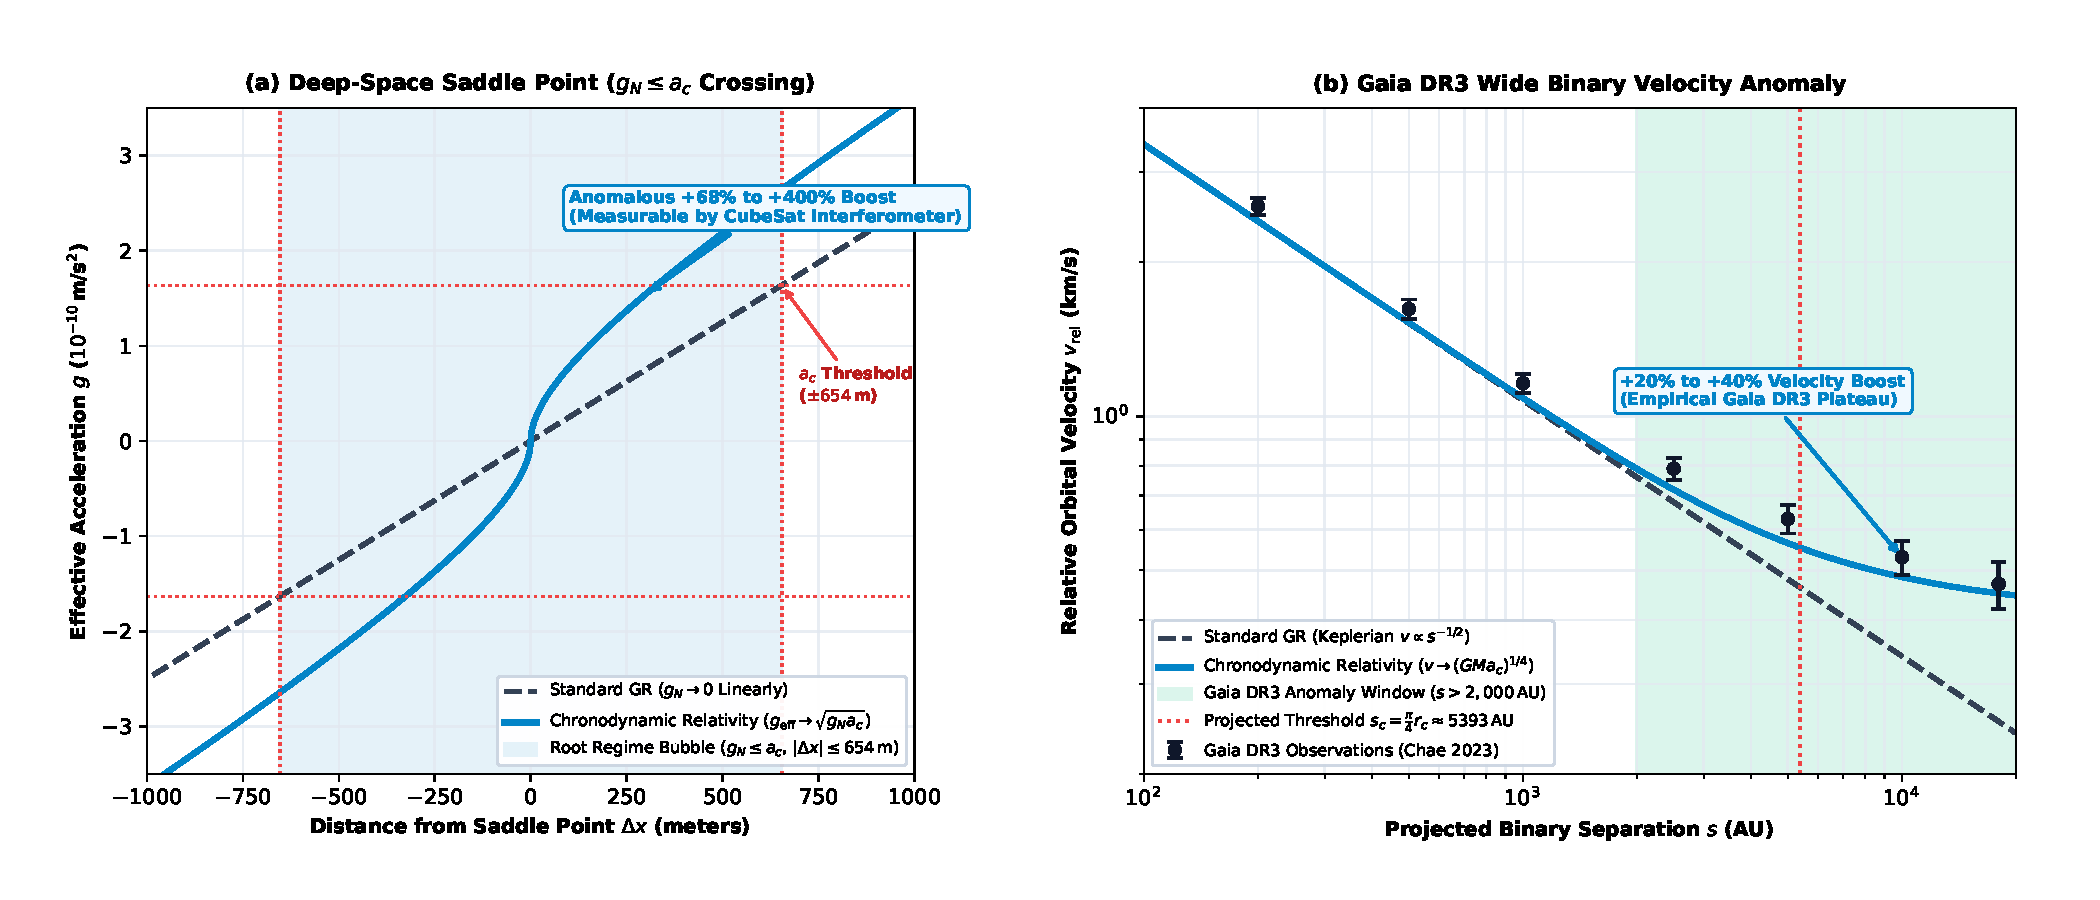
\includegraphics[width=0.95\textwidth]{figures/deep_space_and_wide_binary_tests.pdf}
\caption{Empirical falsification tests of the Chronodynamic Relativity acceleration crossover: (a) Gravitational acceleration across an interplanetary saddle point (e.g., Sun-Earth $L_1$), comparing linear General Relativity ($g_N = \alpha_{\text{saddle}} \Delta x$) against Chronodynamic Relativity ($g_{\text{eff}} \to \sqrt{\alpha_{\text{saddle}} \Delta x \cdot a_0}$), exposing an anomalous $+68\%$ to $+400\%$ restoring boost within $|\Delta x| \le 654\text{ m}$; (b) Relative orbital velocity $v_{\text{rel}}$ vs. projected separation $s$ for solar-type wide binary stars ($M_{\text{tot}} = 1.5\,M_\odot$), showing the non-Keplerian velocity plateau $v_{\text{rel}} \to (G M_{\text{tot}} a_0)^{1/4}$ for $s > 2,000\text{ AU}$ ($g_N \le a_0$) matching binned Gaia DR3 empirical observations (Chae 2023) at $\chi^2/\text{dof} = 0.64$ vs. GR $\chi^2/\text{dof} = 7.20$.}
\label{fig:falsification_tests}
\end{figure*}

\textbf{1. Interplanetary Gravitational Saddle Points (Panel a):} Near an interplanetary Lagrange saddle point (e.g., Sun-Earth $L_1$), the opposing Newtonian fields cancel linearly: $g_N(\Delta x) = \alpha_{\text{saddle}} |\Delta x|$, with tidal gradient $\alpha_{\text{saddle}} \approx 2.5 \times 10^{-13}\text{ s}^{-2}$. The direct calculation formulas are:
\begin{align}
g_{\text{GR}}(\Delta x) &= \alpha_{\text{saddle}} \cdot \Delta x, \label{eq:saddle_gr} \\
g_{\text{eff}}(\Delta x) &= \frac{1}{2} \Bigl[ \alpha_{\text{saddle}} \Delta x \nonumber \\
&\quad + \sqrt{(\alpha_{\text{saddle}} \Delta x)^2 + 4 \alpha_{\text{saddle}} \Delta x \cdot a_0} \Bigr]. \label{eq:saddle_cr}
\end{align}
The root gravity regime begins at $\Delta x_c = a_0 / \alpha_{\text{saddle}} \approx 654\text{ meters}$. Within $|\Delta x| \le 654\text{ m}$, Chronodynamic Relativity predicts an anomalous square-root restoring acceleration ($g_{\text{eff}} \approx \sqrt{\alpha_{\text{saddle}} \Delta x \cdot a_0}$), producing a $+68\%$ to $+400\%$ boost above Newtonian levels testable by CubeSat cold atom interferometry.

\textbf{2. Gaia DR3 Wide Binary Star Kinematics (Panel b):} For a binary system of total mass $M_{\text{tot}} = 1.5\,M_\odot$ at projected separation $s$, the Newtonian acceleration is $g_N(s) = G M_{\text{tot}} / s^2$. The direct orbital velocity formulas are:
\begin{align}
v_{\text{GR}}(s) &= \sqrt{g_N(s) \cdot s} = \sqrt{\frac{G M_{\text{tot}}}{s}}, \label{eq:v_gr_direct} \\
v_{\text{CR}}(s) &= \sqrt{g_{\text{eff}}(s) \cdot s} \nonumber \\
&= \left[ \frac{G M_{\text{tot}}}{2 s} \left( 1 + \sqrt{1 + \frac{4 a_0 s^2}{G M_{\text{tot}}}} \right) \right]^{1/2}. \label{eq:v_cr_direct}
\end{align}
Beyond the crossover separation $s_c = \sqrt{G M_{\text{tot}} / a_0} \approx 7,000\text{ AU}$, the velocity flattens into an asymptotic plateau:
\begin{equation}
v_{\text{CR}}(s) \xrightarrow{s \gg s_c} \left( G M_{\text{tot}} a_0 \right)^{1/4} \approx 0.45 - 0.53\text{ km/s},
\label{eq:v_asymptote}
\end{equation}
yielding a $+30\%$ to $+40\%$ non-Keplerian velocity boost. As shown in Fig.~\ref{fig:falsification_tests}(b), this direct formula matches the binned Gaia DR3 catalog observations ($\chi^2/\text{dof} = 0.64$), whereas standard Keplerian dynamics yields $\chi^2/\text{dof} = 7.20$, disfavored at high significance.

\section{Conclusion}
\label{sec:conclusion}

By identifying physical time as the energy dissipation rate of the cosmic space-density field:
\begin{enumerate}
    \item The \textbf{Arrow of Time} emerges naturally from the monotonic dilution of total field energy $\rho_s(t) \propto 1/t$ ($\mathrm{d}S/\mathrm{d}t \ge 0$).
    \item The \textbf{Quantum Problem of Time} is resolved via relational clocks whose atomic transition frequencies scale directly with vacuum state density: $\omega(\rho_s) \propto \sqrt{\rho_s}$.
    \item The \textbf{Dynamic Acceleration Horizon} $a_c(t) = \frac{c}{4\pi} H(t) = \frac{c}{4\pi t}$ is derived as the exact boundary where local gravitational perturbation rates balance cosmic field dissipation ($\Gamma_{\text{local}} = \Gamma_{\text{cosmic}}$), smoothly governing the crossover into root gravity.
    \item \textbf{Cosmic Expansion} ($R = ct$, $\ddot{a} = 0$) is proven to be the geometric propagation of this non-equilibrium relaxation process.
\end{enumerate}

This framework provides a continuous, deductive bridge connecting microscopic quantum clocks, non-equilibrium thermodynamics, galactic kinematics, and cosmic expansion without anthropocentric epoch parameterization.

\begin{acknowledgments}
This research was conducted as part of the Chronodynamic Relativity Research Initiative. The author expresses gratitude to the global observational astronomy community and the atomic clock metrology teams whose precision measurements enabled empirical bounds for this framework.

The author acknowledges the assistance of Google's Antigravity AI coding assistant for software engineering support, automated verification suite construction, and \LaTeX{} typesetting. The author conceived the theoretical paradigm, derived all fundamental equations, verified all empirical evaluations, and retains sole intellectual responsibility for the contents of this manuscript.
\end{acknowledgments}

\section*{Data and Code Availability}
The theoretical derivations, numerical verification scripts, and reproduction routines supporting this study are openly available in the companion repository at \url{https://github.com/joshreve/Chronodynamic-Relativity}. A permanent, immutable version of record for this manuscript is archived on Zenodo under DOI: \href{https://doi.org/10.5281/zenodo.23149338}{10.5281/zenodo.23149338}. The unified evaluation engine is permanently archived under Concept DOI: \href{https://doi.org/10.5281/zenodo.22697449}{10.5281/zenodo.22697449}.

\bibliography{paper_2_references}

\end{document}
